% Asset ID: A22ConditionalProbabilityTikZ-001
% Purpose: General two-stage conditional probability tree.
\documentclass[tikz,border=10pt]{standalone}
\usepackage{amsmath}
\usepackage{tikz}
\usetikzlibrary{arrows.meta, positioning, calc}
\begin{document}
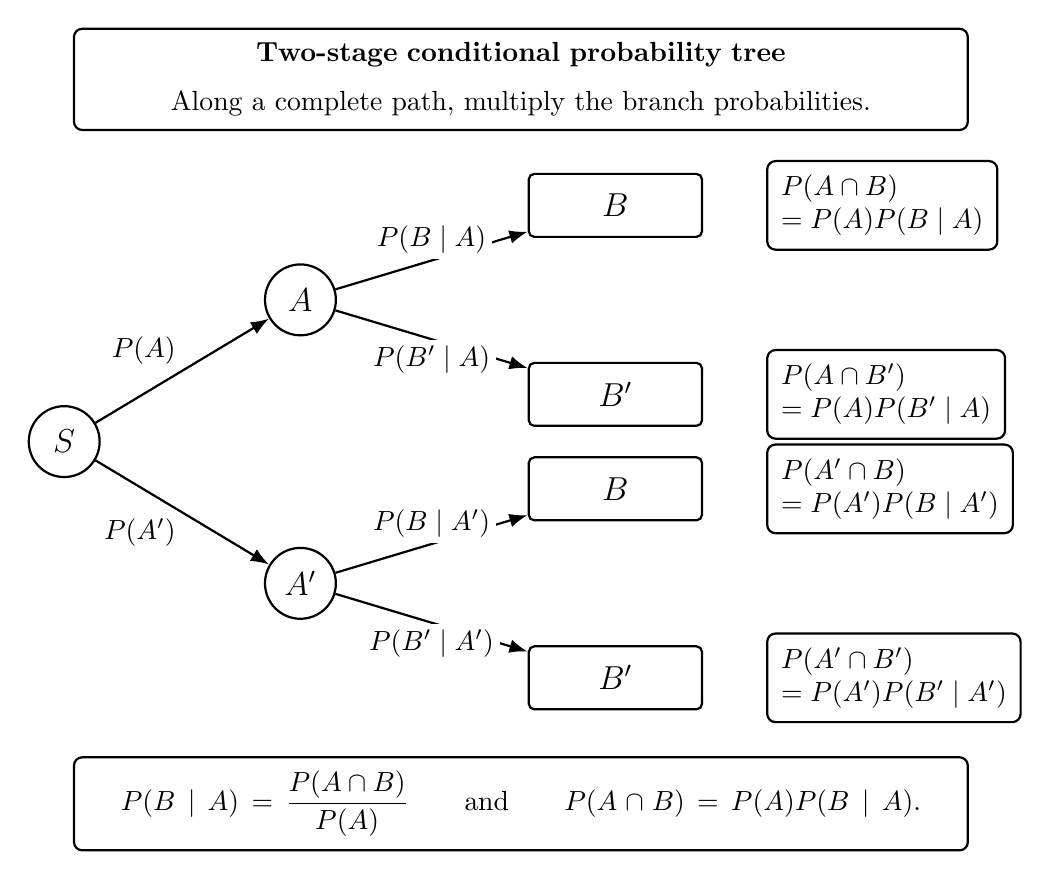
\begin{tikzpicture}[>=Latex,event/.style={circle,draw,thick,minimum size=9mm,font=\large},leaf/.style={rectangle,rounded corners=2pt,draw,thick,minimum width=22mm,minimum height=8mm,font=\large},formula/.style={rectangle,rounded corners=3pt,draw,thick,align=left,inner sep=5pt,font=\normalsize},branchlabel/.style={midway,fill=white,inner sep=2pt,font=\normalsize}]
\node[event] (root) at (0,0) {$S$};
\node[event] (A) at (3,1.8) {$A$};
\node[event] (Ac) at (3,-1.8) {$A'$};
\node[leaf] (AB) at (7,3.0) {$B$};
\node[leaf] (ABc) at (7,0.6) {$B'$};
\node[leaf] (AcB) at (7,-0.6) {$B$};
\node[leaf] (AcBc) at (7,-3.0) {$B'$};
\draw[->,thick] (root)--(A) node[branchlabel,above left] {$P(A)$};
\draw[->,thick] (root)--(Ac) node[branchlabel,below left] {$P(A')$};
\draw[->,thick] (A)--(AB) node[branchlabel,above] {$P(B\mid A)$};
\draw[->,thick] (A)--(ABc) node[branchlabel,below] {$P(B'\mid A)$};
\draw[->,thick] (Ac)--(AcB) node[branchlabel,above] {$P(B\mid A')$};
\draw[->,thick] (Ac)--(AcBc) node[branchlabel,below] {$P(B'\mid A')$};
\node[formula,right=0.8cm of AB] {$P(A\cap B)$\\$=P(A)P(B\mid A)$};
\node[formula,right=0.8cm of ABc] {$P(A\cap B')$\\$=P(A)P(B'\mid A)$};
\node[formula,right=0.8cm of AcB] {$P(A'\cap B)$\\$=P(A')P(B\mid A')$};
\node[formula,right=0.8cm of AcBc] {$P(A'\cap B')$\\$=P(A')P(B'\mid A')$};
\node[formula,align=center,text width=11cm] at (5.8,4.6) {\textbf{Two-stage conditional probability tree}\\[2mm]Along a complete path, multiply the branch probabilities.};
\node[formula,align=center,text width=11cm] at (5.8,-4.6) {$P(B\mid A)=\dfrac{P(A\cap B)}{P(A)}$\qquad and\qquad $P(A\cap B)=P(A)P(B\mid A)$.};
\end{tikzpicture}
\end{document}
